\chapter{Tree}


\section{Binary Tree}
\subsection{Introduction}
\subsection{Basic operations}
\runinhead{Get parent ref.} You can implicitly get a parent reference by return the current recursion function to its parent to maintain the link. Sample code:
\begin{java}
Node deleteMin(Node x) {
    if (x.left == null) return x.right;
    x.left = deleteMin(x.left);
    x.count = 1+size(x.left)+size(x.right);
    return x;
}
\end{java}

\subsection{BST}
\runinhead{Array and BST.}Given either the \textbf{preorder} or \textbf{postorder} (but not inorder) traversal of a BST containing N distinct keys, it is possible to reconstruct the shape of the BST. 

\section{Balanced BST}
\subsection{2-3 Search Tree}
\subsubsection{Insertion}
Insertion into a 3-node at bottom:
\begin{enumerate}
\item Add new key to the 3-node to create a temporary 4-node.
\item Move middle key of the 4-node into the parent (including root's parent).
\item Split the modified 4-node.
\item Repeat recursively up the trees as necessary.
\end{enumerate}
\begin{figure}[hbtp]
\centering
\subfloat{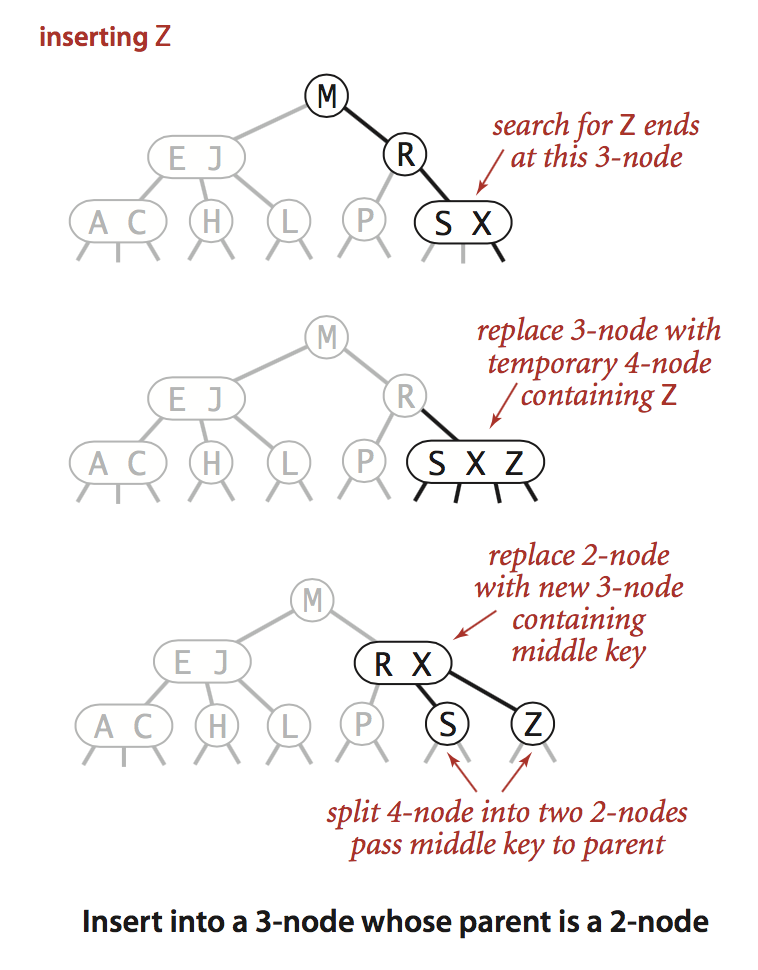
\includegraphics[scale=1.]{23insert1}}
\caption{Insertion 1}
\label{fig:LABEL}
\end{figure}

\begin{figure}[hbtp]
\centering
\subfloat{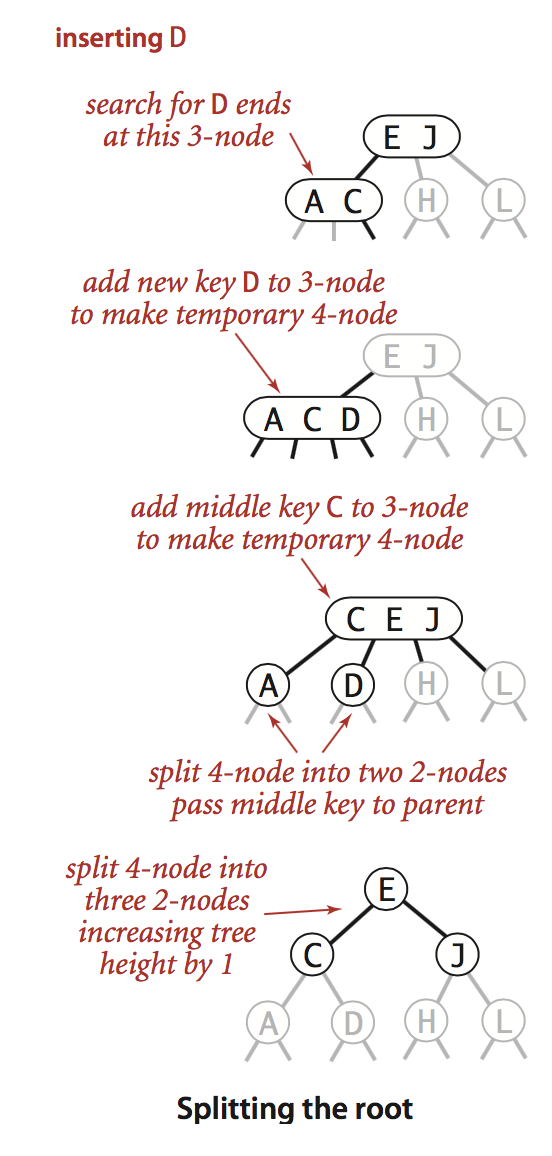
\includegraphics[scale=1.]{23insert2}}
\caption{insert2}
\label{fig:LABEL}
\end{figure}

\subsubsection{Splitting}
Summary of splitting the tree. 
\begin{figure}[hbtp]
\centering
\subfloat{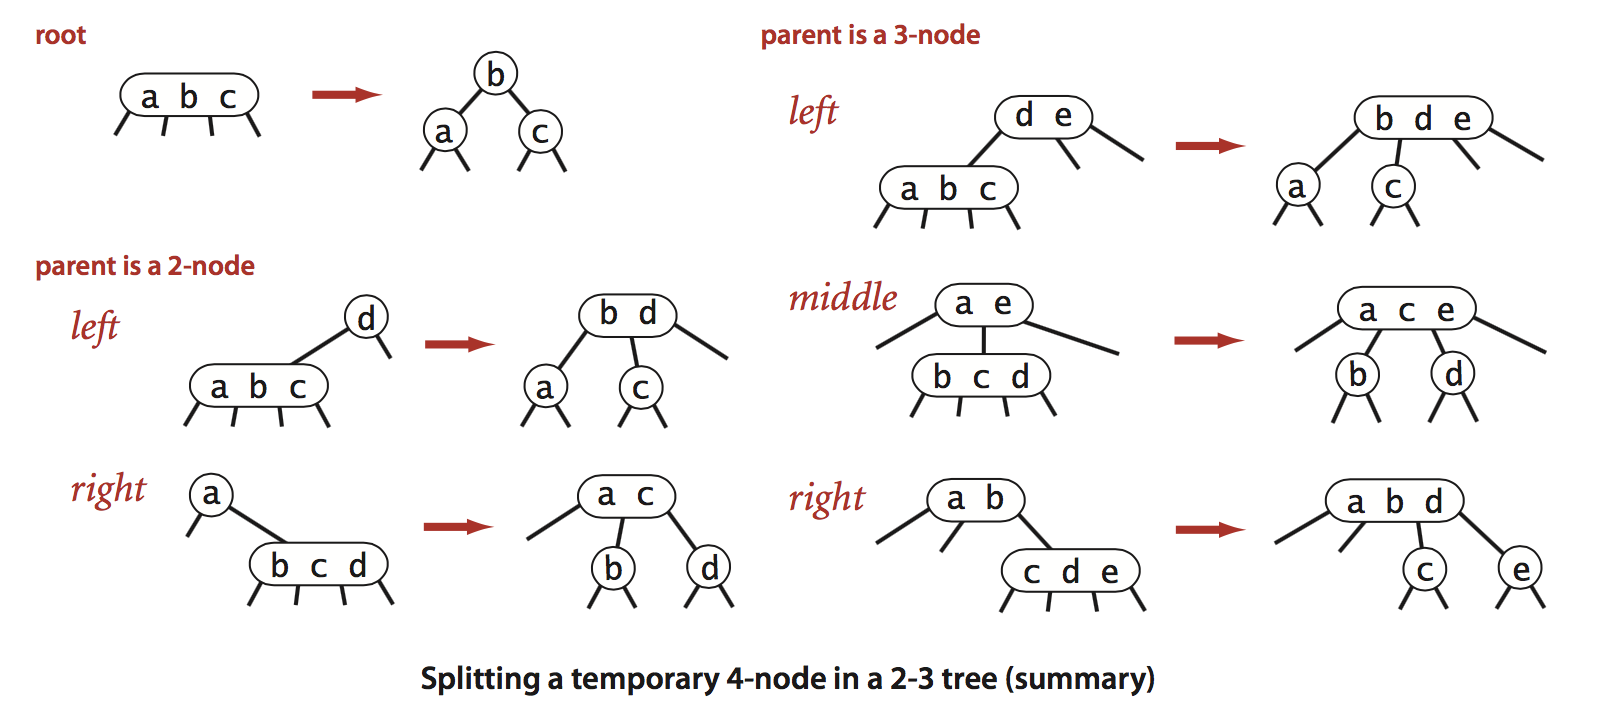
\includegraphics[scale=.60]{23splitting}}
\caption{Splitting temporary 4-ndoe summary}
\label{fig:splitting}
\end{figure}

\subsubsection{Properties}
When inserting a new key into a 2-3 tree, under which one of the following scenarios must the height of the 2-3 tree increase by one? When every node on the search path from the root is a 3-node

\subsection{Red-Black Tree}

\section{Segment Tree}
\subsection{Introduction}
The structure of \textbf{Segment Tree} is a binary tree which each node has two attributes start and end denote an segment/interval. Notice that by practice, the interval is normally $[start, end)$ but sometimes it can be $[start, end]$, which depends on the question definition. 

Structure:  
\begin{lstlisting}[columns=flexible]
                     [0, 4, count=3]
                     /             \
          [0,2,count=1]             [2,4,count=2]
          /         \               /            \
   [0,1,count=1] [1,2,count=0] [2,3,count=1], [3,4,count=1]
\end{lstlisting}

Variants:
\begin{enumerate}
\item Sum Segment Tree.
\item Min/Max Segment Tree.
\item Count Segment Tree. 
\end{enumerate}

For a \textbf{Maximum Segment Tree}, which each node has an extra value max
to store the maximum value in this node's interval.

\subsection{Operations}
Components in Segment Tree:
\begin{enumerate}
\item Build
\item Query 
\item Modify 
\end{enumerate}

Notice:
\begin{enumerate}
\item Only build need to change the start and end recursively.
\item Pre-check is preferred in recursive calls.
\end{enumerate}


Code:
\begin{python}
DEFAULT = 0
f = lambda x, y: x+y


class Node(object):
    def __init__(self, start, end, m):
        self.start, self.end, self.m = start, end, m
        self.left, self.right = None, None


class SegmentTree(object):
    def __init__(self, A):
        self.A = A
        self.root = self.build_tree(0, len(self.A))

    def build_tree(self, s, e):
        """
        segment: [s, e)
        """
        if s >= e:
            return None

        if s+1 == e:
            return Node(s, e, self.A[s])

        left = self.build_tree(s, (s+e)/2)
        right = self.build_tree((s+e)/2, e)
        val = DEFAULT
        if left: val = f(val, left.m)
        if right: val = f(val, right.m)
        root = Node(s, e, val)
        root.left = left
        root.right = right

        return root

    def query(self, root, s, e):
        """
        :type root: Node
        """
        if not root:
            return DEFAULT

        if s <= root.start and e >= root.end:
            return root.m

        if s >= root.end or e <= root.start:
            return DEFAULT

        l = self.query(root.left, s, e)
        r = self.query(root.right, s, e)
        return f(l, r)

    def modify(self, root, idx, val):
        """
        :type root: Node
        """
        if not root or idx >= root.end or idx < root.start:
            return

        if idx == root.start and idx == root.end-1:
            root.m = val
            self.A[idx] = val
            return

        self.modify(root.left, idx, val)
        self.modify(root.right, idx, val)
        val = DEFAULT
        if root.left: val = f(val, root.left.m)
        if root.right: val = f(val, root.right.m)
        root.m = val
\end{python}
\section{Balanced Tree}

\subsection{AVL Tree}

\subsection{Red-Black Tree}

\subsection{Summarizing properties}


